\input{configuration}

\title{Lecture 9 --- Algorithms, Concurrency, and Parallelism }

\author{Jeff Zarnett \& Patrick Lam \\ \small \texttt{jzarnett@uwaterloo.ca}, \texttt{patrick.lam@uwaterloo.ca}}
\institute{Department of Electrical and Computer Engineering \\
  University of Waterloo}
\date{\today}

\begin{document}

\begin{frame}
  \titlepage

 \end{frame}

\part{Algorithms}
\begin{frame}[fragile]
\partpage
\begin{center}
	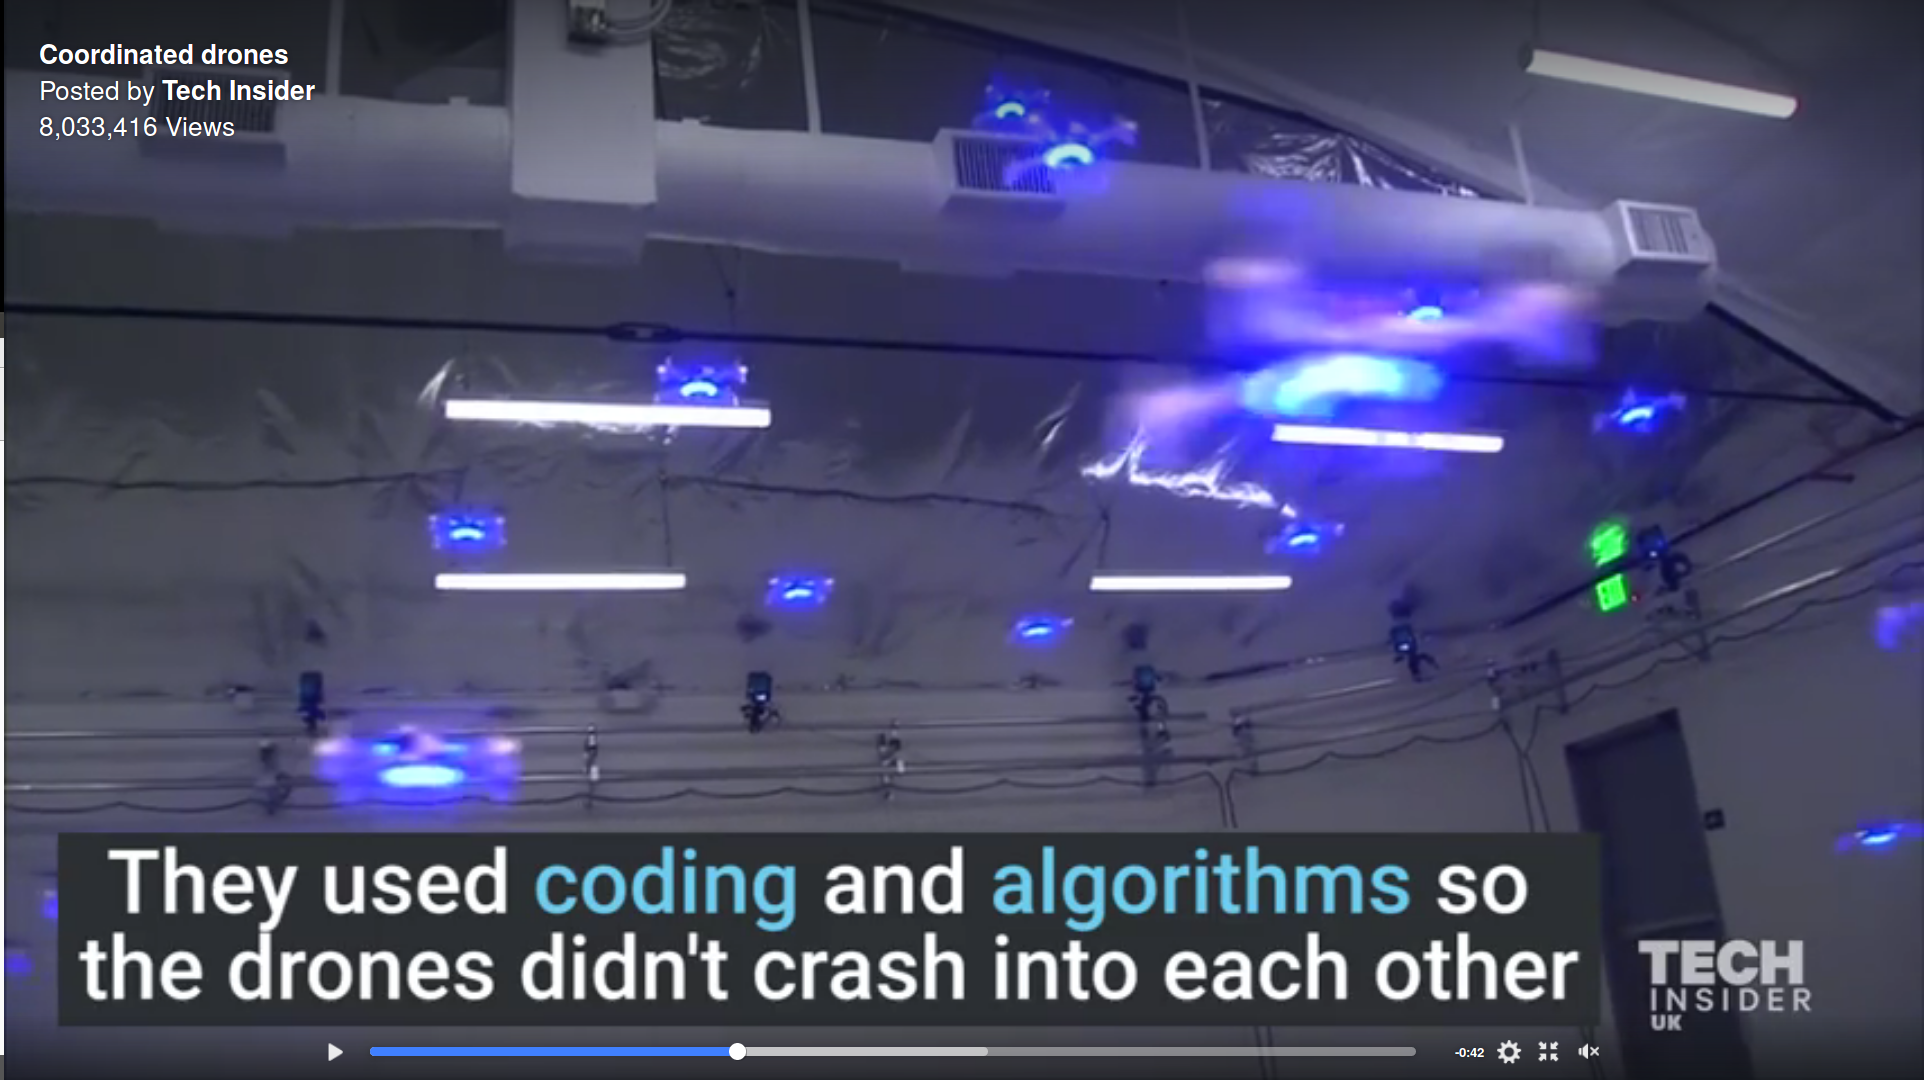
\includegraphics[width=0.4\textwidth]{images/coding-algorithms.png}\\
	
	\begin{lstlisting}
if(goingToCrashIntoEachOther) { 
  dont(); 
}
\end{lstlisting}
	
\end{center}
\end{frame}

\begin{frame}
\frametitle{Algorithmic Complexity}

Remember we often care about worst-case run-time performance:

\begin{center}
	\includegraphics[width=0.6\textwidth]{images/big-o-complexity}
\end{center}

But you know this already!\\
\quad You're not here to hear me tell you to use Quicksort instead of Bubblesort.

\end{frame}

\begin{frame}
\frametitle{Is Sorting a Bad Example?}
In reality, you use a library- or language-provided sort.

That is, just call \texttt{.sort()} on the collection and it's done!

Ah, but what about... \alert{leetcode}?

\end{frame}

\begin{frame}
\frametitle{Just Grind Leetcode and Git Gud}

\begin{center}
	
\includegraphics[width=0.8\textwidth]{images/leetcode.jpg}
\end{center}

Is this how to get a job these days? (Spoiler alert: often.)

\end{frame}

\begin{frame}
\frametitle{Good Ideas in the Grind}
There are some ideas from how to grind leetcode that help in other situations.

More time is likely to be spent on architecture or understanding requirements.


But let's take some ideas from what I tell people for interview prep.
\end{frame}

\begin{frame}
\frametitle{Start with Simple}

\begin{center}
	
\includegraphics[width=0.4\textwidth]{images/bruteforce.jpg}
\end{center}

In many (non-leetcode) scenarios, simple and correct suffices!\\
\quad Either $n$ is small enough or this code is not performance-critical.

\end{frame}

\begin{frame}
\frametitle{Next Step: Refine}
Refine is improve what you've got. See \textit{Cracking the Coding Interview} for more!

Look for:\\
\begin{itemize}
	\item Bottlenecks
	\item Unnecessary Work
	\item Duplicated Work
\end{itemize}

\end{frame}

\begin{frame}
\frametitle{Use the Force, Luke}

In a coding-interview, you have a well-defined set of pieces of information.\\
\quad Chances are, you need to use all of them to find optimal solution.

In other situations, it may not be provided; investigate!

You may need to be the change you want to see.

\end{frame}

\begin{frame}
\frametitle{Other Thoughts}

Big-O complexity assumes a large enough $n$ that the other terms don't matter. 

That's fine for an interview, but is not always true in real life. 

Sorting a large array or putting it into a Hashmap is likely to be optimal if you intend to use it many times, but maybe is not worthwhile if we search once.
\end{frame}

\begin{frame}
\frametitle{Ask for Help}

\begin{center}
	
\includegraphics[width=0.4\textwidth]{images/askforhelp.png}
\end{center}

\end{frame}

\begin{frame}
\frametitle{Algorithmic Improvements Limits}

Remember also that algorithmic complexity improvements always have limits.

To successfully mark the final exam, the teaching team really does have to look at every question of every exam paper. 

No amount of cleverness in the process can get around the fact that the only way to properly mark the exam is to look at every answer from each student.

\end{frame}

\begin{frame}
\frametitle{Accidentally Quadratic}
Many problems really are linear at the core; a problem arises when we combine two linear things and get quadratic behaviour. 


Oh no! This is a situation that can be described as ``accidentally quadratic''.

\begin{center}
	
\includegraphics[width=0.4\textwidth]{images/accidents.jpg}
\end{center}


\end{frame}

\begin{frame}
\frametitle{Older Code, But it Checks Out}
The 2019 Rust-specific example is about Robin-Hood Hashing.

Remember open addressing and linear probile?

Moving the data to a new hash table is a problem...

\end{frame}

\begin{frame}
\frametitle{Loop-and-Loop}
Copy the data to a table half the size of the original.

As it gets close to full: quadratic behaviour!\\
\quad Linear for each element in $1^{st}$ table, linear to find a free space in $2^{nd}$.

\begin{center}
  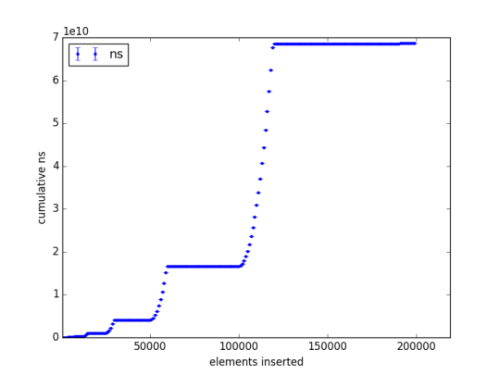
\includegraphics[width=0.5\textwidth]{images/robinhoodhashing.png}
\end{center}

\end{frame}

\begin{frame}
\frametitle{Sometimes is Always}
Algorithmic analysis is, remember, often worst-case scenario.

Don't over-index on this example:\\
\begin{center}
	
\includegraphics[width=0.3\textwidth]{images/well-actually.png}
\end{center}

It just means that sometimes the normally-best approach isn't best this time.

\end{frame}

\begin{frame}
\frametitle{Hello Marking, My Old Friend}
If we can't do any better than linear (or maybe even quadratic), what do we do?

The exam marking example gives a hint: divide \& conquer!

Or, in other words, parallelism.

\end{frame}

\part{Parallelism}

\begin{frame}
\partpage
\end{frame}


\begin{frame}
  \frametitle{Parallelism versus Concurrency}

  Before we talk about parallelism, let's distinguish it from concurrency.

  {\bf Parallelism}

  Two or more tasks are \structure{parallel}\\ \hspace*{2em} if they are running at the same time. 

  Main goal: run tasks as fast as possible. 

  Main concern: \structure{dependencies}.
  \vfill
  {\bf Concurrency}

  Two or more tasks are \structure{concurrent}\\ \hspace*{2em} if the ordering of the two tasks is not 
  predetermined. 

  Main concern: \structure{synchronization}.

\end{frame}

\begin{frame}
  \frametitle{Limitations of Speedups}

    Our main focus is parallelization.\\[1em]
  \begin{itemize}
    \item Most programs have a sequential part and a parallel part; and,\\[1em]
    \item Amdahl's Law answers, ``what are the limits to parallelization?''
  \end{itemize}
  
  \begin{center}
	\includegraphics[width=0.7\textwidth]{images/linedrawnhere.jpeg}
\end{center}

\end{frame}



\begin{frame}
\frametitle{Visualizing Amdahl's Law}

  \hspace*{2em}\begin{minipage}{.8\textwidth}
  $S$: fraction of serial runtime in a serial execution.

  $P$: fraction of parallel runtime in a serial execution.

  Therefore, $S + P = 1$.\\[2em]

  With 4 processors, best case, what can happen to the following runtime?
  \end{minipage}

  \hspace*{5em}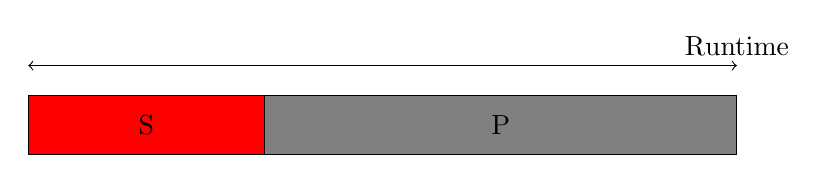
\begin{tikzpicture}
   \draw[<->] (-1.5,0.75) -- (7.5,0.75) node[above] {Runtime};
   \draw (0,0) node[rectangle, fill=red, minimum height=0.75cm, minimum width=3cm,draw] {S};
   \draw (4.5,0) node[rectangle, fill=gray, minimum height=0.75cm, minimum width=6cm,draw] {P};
  \end{tikzpicture}
\end{frame}

\begin{frame}
  \frametitle{Visualizing Amdahl's Law}

  \hspace*{5em}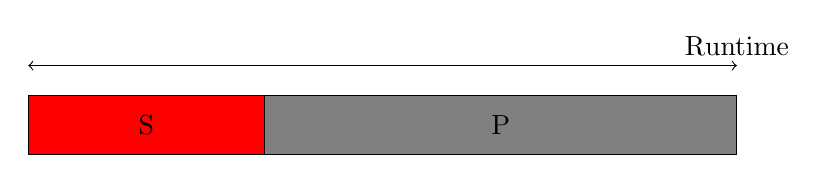
\begin{tikzpicture}
   \draw[<->] (-1.5,0.75) -- (7.5,0.75) node[above] {Runtime};
   \draw (0,0) node[rectangle, fill=red, minimum height=0.75cm, minimum width=3cm,draw] {S};
   \draw (4.5,0) node[rectangle, fill=gray, minimum height=0.75cm, minimum width=6cm,draw] {P};
  \end{tikzpicture}
  \vfill
  We want to split up the parallel part over 4 processors
  \vfill
  \hspace*{5em}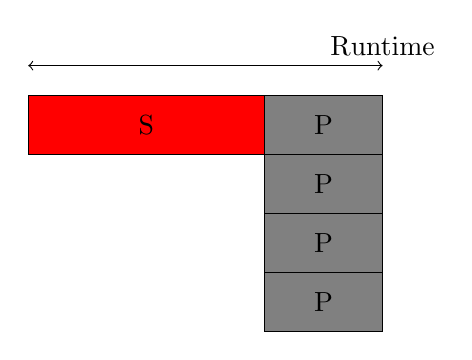
\begin{tikzpicture}
   \draw[<->] (-1.5,0.75) -- (3,0.75) node[above] {Runtime};
   \draw (0,0) node[rectangle, fill=red, minimum height=0.75cm, minimum width=3cm,draw] {S};
   \draw (2.25,0) node[rectangle, fill=gray, minimum height=0.75cm, minimum width=1.5cm,draw] {P};
   \draw (2.25,-0.75) node[rectangle, fill=gray, minimum height=0.75cm, minimum width=1.5cm,draw] {P};
   \draw (2.25,-1.5) node[rectangle, fill=gray, minimum height=0.75cm, minimum width=1.5cm,draw] {P};
   \draw (2.25,-2.25) node[rectangle, fill=gray, minimum height=0.75cm, minimum width=1.5cm,draw] {P};
  \end{tikzpicture}
\end{frame}

\begin{frame}
  \frametitle{Obey the Law}

\Large
$T_s$: time for the program to run in serial

$N$: number of processors/parallel executions

$T_p$: time for the program to run in parallel
\vfill
  \begin{itemize}
    \item Under perfect conditions, get $N$ speedup for $P$
  \end{itemize}
\vfill

  \begin{center}
$T_p = T_s \cdot (S + \frac{P}{N})$
  \end{center}
\end{frame}

\begin{frame}
  \frametitle{Obey the Law}

  \hspace*{3em} How much faster can we make the program?

  \begin{eqnarray*}
  \mbox{\em speedup} &=& \frac{T_s}{T_p}\\
                     &=& \frac{T_s}{T_S \cdot (S + \frac{P}{N})}\\
                     &=& \frac{1}{S + \frac{P}{N}}
  \end{eqnarray*}
  \vfill
  \hspace*{3em} (assuming no overhead for parallelizing; or costs near
  zero)

\end{frame}

\begin{frame}
  \frametitle{Fixed-Size Problem Scaling, \\ Varying Fraction of Parallel Code}

  \begin{center}
    \hspace*{2em}\includegraphics[scale=0.68]{images/parallel-scaling.pdf}
  \end{center}
\end{frame}


\begin{frame}
  \frametitle{Amdahl's Law}

 \hspace*{2em}Replace $S$ with $(1 - P)$:

  \begin{center}
    \structure{$\mbox{\em speedup} = \frac{1}{(1 - P) + \frac{P}{N}}$}
  \end{center}
  \vfill
  \begin{center}
    $\mbox{\em maximum speedup} = \frac{1}{(1 - P)}$, since $\frac{P}{N} \rightarrow 0$
  \end{center}

As you might imagine, the asymptotes in the previous graph are bounded by the
  maximum speedup.
\end{frame}

\begin{frame}
\frametitle{Speedup Example}


Suppose: a task that can be executed in 5~s, containing a parallelizable loop.

Initialization and recombination code in this routine requires 400~ms. 

So with one processor executing, it would take about 4.6~s to execute the loop. 

Split it up and execute on two processors: about 2.3~s to execute the loop. 

Add to that the setup and cleanup time of 0.4~s and we get a total time of 2.7~s. 

Completing the task in 2.7~s rather than 5~s represents a speedup of about~46\%.

\end{frame}


\begin{frame}
\frametitle{Amdahl's Law on the 5~s Task}

Applying this formula to the example:

\begin{center}
	\begin{tabular}{r|l}
	\textbf{Processors} & \textbf{Run Time (s)} \\ \hline
	1 & 5\\
	2 & 2.7\\
	4 & 1.55\\
	8 & 0.975\\
	16 & 0.6875 \\
	32 & 0.54375 \\
	64 & 0.471875 \\
	128 & 0.4359375\\
	\end{tabular}
\end{center}

\end{frame}

 
\begin{frame}
\frametitle{Observations on the 5~s Task}

1. Diminishing returns as we add more processors.

2. Converges on 0.4~s.

The most we could speed up this code is by a factor of $\frac{5}{0.4}\approx 12.5$.

But that would require infinite processors (and therefore infinite money).

\end{frame}

\begin{frame}
  \frametitle{Assumptions behind Amdahl's Law}

    We assume:
    \begin{itemize}
    \item problem size is fixed (we'll see this soon);
    \item program/algorithm behaves the same on 1 processor and on $N$ processors;
    \item that we can accurately measure runtimes---\\ ~~i.e. that overheads don't matter.
    \end{itemize}
    
    \begin{center}
	\includegraphics[width=0.6\textwidth]{images/overhead.jpg}
	\end{center}
  
\end{frame}

\begin{frame}
  \frametitle{Amdahl's Law Generalization}

  \hspace*{2em} The program may have many parts, each of which we can tune to
  a different degree.\\[1em]

  Let's generalize Amdahl's Law.\\[1em]

  $f_1, f_2, \ldots, f_n$: fraction of time in part $n$

  $S_{f_1}, S_{f_n}, \ldots, S_{f_n}$: speedup for part $n$

  \vfill
  \begin{center}
  \structure{\[\mbox{\em speedup} = \frac{1}{\frac{f_1}{S_{f_1}} + \frac{f_2}{S_{f_2}} + \ldots +
    \frac{f_n}{S_{f_n}}}\]}
  \end{center}
\end{frame}


\begin{frame}
  \frametitle{Application (1)}

  \hspace*{2em} 
Consider a program with 4 parts in the following scenario:\\[2em]
    \begin{tabular}{r|r|r|r}
    \multicolumn{2}{l}{} & \multicolumn{2}{c}{Speedup} \\
    Part & Fraction of Runtime & Option 1 & Option 2\\
    \hline
    1 & 0.55 & 1  & 2\\
    2 & 0.25 & 5  & 1\\
    3 & 0.15 & 3  & 1\\
    4 & 0.05  & 10 & 1\\
  \end{tabular}

~\\[2em]
  We can implement either Option 1 or Option 2. \\
  Which option is better?

\end{frame}

\begin{frame}
  \frametitle{Application (2)}


  \hspace*{2em} ``Plug and chug'' the numbers:\\[1em]

  {\bf Option 1} \vspace*{-2em}

  \[ \mbox{\em speedup} = \frac{1}{0.55 + \frac{0.25}{5} + \frac{0.15}{3} + \frac{0.05}{5}}
    = 1.53  \]
~\\[1em]
  {\bf Option 2} \vspace*{-2em}

   \[\mbox{\em speedup} = \frac{1}{\frac{0.55}{2} + 0.45} = 1.38 \hspace*{5.5em}\]


\end{frame}

\begin{frame}
  \frametitle{Empirically estimating parallel speedup P}

  \hspace*{2em} Useful to know, don't have to commit to memory:
  \vfill
  \[P_{\mbox{\scriptsize estimated}} = \frac{\frac{1}{\mbox{\em speedup}}-1}{\frac{1}{N}-1}\]
  \vfill
  \hspace*{2em} \begin{minipage}{.8\textwidth} \begin{itemize}
    \item Quick way to guess the fraction of parallel code
    \item Use $P_{\mbox{\scriptsize estimated}}$ to predict speedup for a different number of processors
  \end{itemize} \end{minipage}
\end{frame}

\begin{frame}
  \frametitle{Summary of Amdahl's Law}

\hspace*{2em} Important to focus on the part of the program with most impact.\\[1em]

\hspace*{2em} Amdahl's Law:\\[1em]
\hspace*{2em}
  \begin{itemize}
    \item estimates perfect performance gains from
          parallelization (under assumptions); but,
    \vfill
    \item only applies to solving a \structure{fixed problem size} in the
          shortest possible period of time
  \end{itemize}
\end{frame}

\begin{frame}
  \frametitle{Gustafson's Law: Formulation}

\hspace*{2em} 
\begin{tabbing}
  $n$:~~~~~~ \= problem size\\[.1em]

  $S(n)$:~~ \> fraction of serial runtime for a parallel execution\\[.1em]

  $P(n)$:~~ \> fraction of parallel runtime for a parallel execution\\
\end{tabbing}


\begin{eqnarray*}
T_p &=& S(n) + P(n) = 1 \\
T_s &=& S(n) + N \cdot P(n) 
\end{eqnarray*}

\[ \mbox{\em speedup} = \frac{T_s}{T_p} \]
\end{frame}

\begin{frame}
  \frametitle{Gustafson's Law}

\hspace*{2em}
  \structure{$speedup = S(n) + N \cdot P(n)$}\\[1em]

  Assuming the fraction of runtime in serial part decreases as $n$ increases,
  the speedup approaches $N$.


Yes! Large problems can be efficiently parallelized. (Ask Google.)

\end{frame}

\begin{frame}
  \frametitle{Driving Metaphor}

  {\bf Amdahl's Law}
  
  Suppose you're travelling between 2 cities 90~km apart. If you travel for an
  hour at a constant speed less than 90 km/h, your average will never equal
  90~km/h, even if you energize after that hour.
  \vfill
  {\bf Gustafson's Law}

  Suppose you've been travelling at a constant speed less than 90~km/h. Given
  enough distance, you can bring your average up to 90~km/h.
\end{frame}

\part{Parallelization Techniques}
\begin{frame}
\partpage
\begin{center}
	\includegraphics[width=0.25\textwidth]{images/cutup.jpg}
\end{center}
\end{frame}

\begin{frame}
\frametitle{Lock It Down}
The more locks and locking we need, the less scalable the code is going to be. 

You may think of the lock as a resource. 
The more threads or processes that are looking to acquire that lock, the more ``resource contention'' we have.

And thus more waiting and coordination are going to be necessary.

\end{frame}

\begin{frame}
\frametitle{``We have a new enemy...''}

Assuming we're not working with an embedded system where all memory is statically allocated in advance, there will be dynamic memory allocation. 

The memory allocator is often centralized and may support only one thread allocating or deallocating at a time (using locks to ensure this). 

This means it does not necessarily scale very well.

There are some techniques for dynamic memory allocation that allow these things to work in parallel.


\end{frame}


\begin{frame}
\frametitle{Everybody Into the Pool}

If we have a pool of workers, the application just submits units of work, and then on the other side these units of work are allocated to workers. 

The number of workers will scale based on the available hardware. 

This is neat as a programming practice: as the application developer we don't care quite so much about the underlying hardware. 

Let the operating system decide how many workers there should be, to figure out the optimal way to process the units of work.

\end{frame}


\begin{frame}[fragile]
\frametitle{Rust Thread Pool}

\begin{lstlisting}[language=Rust]
use std::collections::VecDeque;
use std::sync::{Arc, Mutex};
use threadpool::ThreadPool;
use std::thread;

fn main() {
    let pool = ThreadPool::new(8);
    let queue = Arc::new(Mutex::new(VecDeque::new()));
    println!("main thread has id {}", thread_id::get());

    for j in 0 .. 4000 {
        queue.lock().unwrap().push_back(j);
    }
    queue.lock().unwrap().push_back(-1);
\end{lstlisting}


\end{frame}
\begin{frame}[fragile]
\frametitle{Rust Thread Pool}

\begin{lstlisting}[language=Rust]
    for i in 0 .. 4 {
        let queue_in_thread = queue.clone();
        pool.execute(move || {
            loop {
                let mut q = queue_in_thread.lock().unwrap();
                if !q.is_empty() {
                    let val = q.pop_front().unwrap();
                    if val == -1 {
                        q.push_back(-1);
                        println!("Thread {} got the signal to exit.", thread_id::get());
                        return;
                    }
                    println!("Thread {} got: {}!", thread_id::get(), val);
                }
            }
        });
    }
    pool.join();
}
\end{lstlisting}


\end{frame}


\begin{frame}[fragile]
\frametitle{Thread Pool Output}


\begin{verbatim}
main thread has id 4455538112
Thread 123145474433024 got: 0!
Thread 123145474433024 got: 1!
Thread 123145474433024 got: 2!

...

Thread 123145478651904 got: 3997!
Thread 123145478651904 got: 3998!
Thread 123145478651904 got: 3999!
Thread 123145476542464 got the signal to exit.
Thread 123145484980224 got the signal to exit.
Thread 123145474433024 got the signal to exit.
Thread 123145478651904 got the signal to exit.
\end{verbatim}


\end{frame}

\end{document}

